\chapter{绪论}
\section{课题背景}

稀疏下三角矩阵求解(Sparse Triangular Solve, SpTRSV)并行算法是很多数值计算方法的重要组成部分,比如用直接法求解稀疏矩阵的线性方程组\cite{davis2006direct},迭代法求解稀疏矩阵的预条件子\cite{elman1982iterative},以及最小二乘法的求解\cite{saad2003iterative},是现代科学计算中一个广泛使用的计算核心,在数值模拟计算中,通常会使用迭代法或直接法求解大规模稀疏线性方程组,而SpTRSV的效率直接影响了线性方程组的求解效率,故提高SpTRSV算法的性能至关重要。

相比于稠密下三角举证解法器\cite{hogg2013fast}或者其他稀疏矩阵计算方法,例如稀疏矩阵转置\cite{wang2016parallel},稀疏矩阵向量乘法\cite{liu2015csr5}\cite{liu2015speculative},和稀疏矩阵乘法\cite{liu2015framework},SpTRSV频繁且离散地数据访存、任务之间存在着很强的依赖、需要细粒度的同步、任务之间负载不均衡等特点是并行优化更加难以进行。

SpTRSV算法主要是从方程组$Lx=b$中求解未知数向量$ x $,其中$ L $是下三角矩阵,且对角线上的元素都不为0。因为这意味这要计算其中的一个未知数$x_k$,需要先计算出其前置未知数$x_0$, \dots, $x_{k-1}$ 中的一个子集。这些任务间的依赖关系,就使得SpTRSV的计算转换成了一个任务依赖图的计算(Task Dependent Graph,TDG),而且这个TDG是一张有方无环图(Directed Acyclic Graph)。

华为作为鲲鹏计算产业的成员,聚焦于发展华为鲲鹏+昇腾双引擎芯片族,通过“硬件开放、软件开源、使能合作伙伴”来推动计算产业的发展。华为鲲鹏920处理器兼容了ARMv8架构。最多拥有64核心。其浮点及SIMD运算单元支持每拍2条ARM Neon 128bits浮点运算。华为鲲鹏系统支持NUMA内存架构,实现最多4个鲲鹏920互联和最高256个物理核的NUMA架构。 

稀疏矩阵运算在科学计算、数据分析、机器学习等应用中十分常见,而稀疏矩阵频繁且离散地数据访存、任务之间存在着很强的依赖、需要细粒度的同步、任务之间负载不均衡等特点又给代码优化带来了巨大的挑战。


\section{研究现状}

\begin{figure}[htbp]
    \centering
    \subfigure[下三角矩阵]{
    \begin{minipage}[t]{0.25\linewidth}
    \centering
    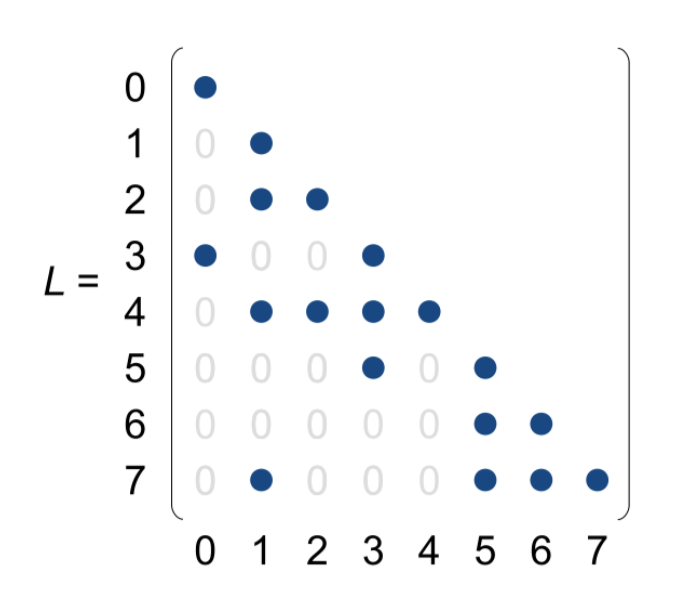
\includegraphics[height=1.3in]{Sparse_Matrix.png}
    \end{minipage}%
    }%
    \subfigure[任务依赖图]{
    \begin{minipage}[t]{0.25\linewidth}
    \centering
    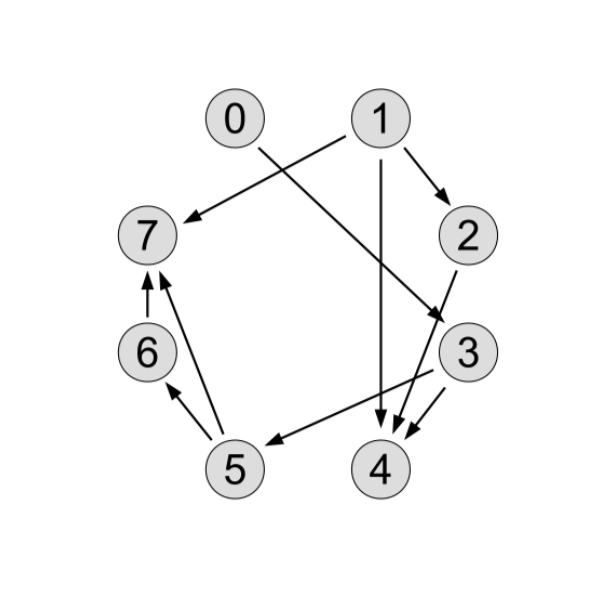
\includegraphics[height=1.3in]{DAG.png}
    \label{TDG}
    \end{minipage}%
    }%
    \subfigure[level-sets]{
    \begin{minipage}[t]{0.25\linewidth}
    \centering
    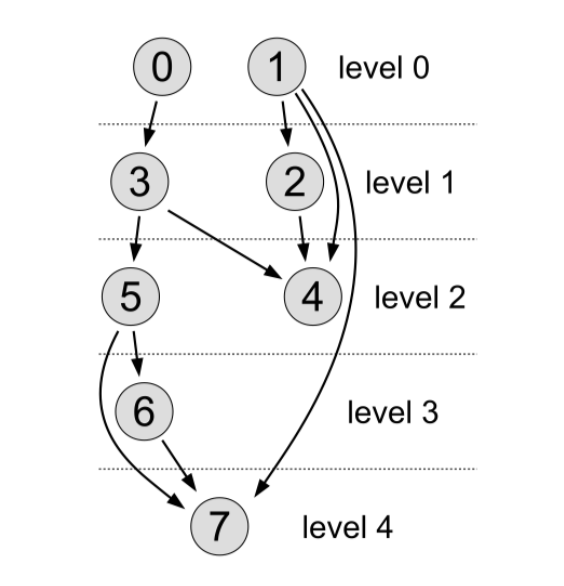
\includegraphics[height=1.3in]{level-sets.png}
    \end{minipage}
    \label{level-sets}
    }%
    \centering
\end{figure}

有研究者Saad\cite{anderson1989solving},以及Saltz\cite{saltz1990aggregation}根据SpTRSV算法是一张任务依赖图\ref{TDG}的特点,提出了基于level-sets的方法,在预处理阶段构建一个任务依赖图,如图\ref{level-sets},之后就可以在level内部进行并行,在level之间设置同步屏障,一个level执行完了再执行下一个level。

随后有研究人员在体系结构层面上针对CPU\cite{kabir2015sts}\cite{park2014sparsifying}\cite{Schreiber1982}\cite{wolf2010factors}以及GPU\cite{li2013gpu}\cite{naumov2011parallel}\cite{suchoski2012adapting}进行了优化。

基于level-sets的算法,存在着两个缺陷:第一,虽然可以在每个level上进行并行取得良好的并行度,但是需要在预处理阶段构建一个TAG图,计算每个任务的level,以及处理任务之间任务负载均衡的问题。然而,在预处理阶段往往会花费大量的时候,写出一个有良好扩展性的并行预处理算法同样具有挑战性,往往可能会导致预处理的时间远远大于并行计算任务图的时间,甚至在计算任务图上获得的加速甚至不能抵消预处理阶段产生的计算时间。第二,基于level-sets的的算法需要在每个level之间都要使用一个屏障确保进行同步,等待该level内的任务都执行完了再继续下个一个任务,在负载不均衡的情况下,这会产生大量的等待时间,随着核心数量的上升该同步方式的开销也会随之上升。

面对以上两个level-sets的缺陷,有研究人员提出了以下的优化算法。

Jongsoo Park\cite{park2014sparsifying}在基于level-sets算法进行了一些优化。他发现传统的基于level-sets的算法所使用的屏障式的同步方式会产生大量的开销。因此作者提出了一种peer-to-peer的同步方式。线程在任务执行完了之后不再是等待在屏障处,等待其他线程执行到该屏障处,而是会判断下一个任务的前置需求是否被完成,如果已经完成了,那么就继续运行下去。相比于基于屏障的同步方式,peer-to-peer的同步方式具有更好的扩展性。

在减少同步所需消耗方面,作者还发现,在SpTRSV算法的任务依赖图中,大部分的依赖都是多余的,作者期望通过一步预处理操作来删除这些多余依赖。例如在 2→3→5 和 2→5 这种边存在的情况下,删除了 2→5 这条边。另一方面,作者发现在这些多余依赖当中,大部分都是两跳的(比如上述的 2→5 这条边),少部分是三跳或者三跳以上。为了减少预处理的计算量,作者选择用粗略但快速的算法,只删除两跳的依赖边,而不是删除所有的多余依赖。减少了大约90\%的多余依赖,具体效果如\ref{sparsifying_edge}。该算法运行在12核的Xeon处理器上,相比于传统的基于level-sets以及屏障式同步的算法获得了至少1.6倍的加速比。

\begin{figure}[htbp]
    \centering
    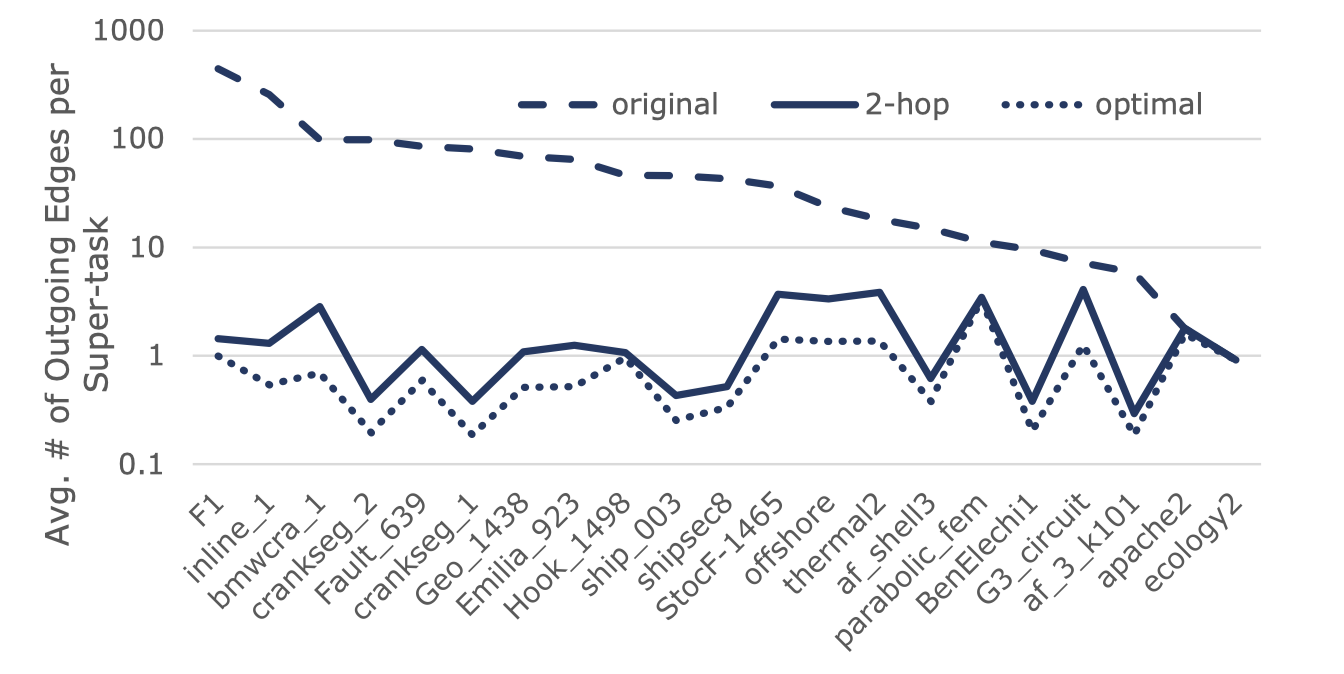
\includegraphics[width=0.7\textwidth]{sparsifying_edge.png}
    \caption{每个super-task的出度有了显著的减少}
    \label{sparsifying_edge}
\end{figure}

同时作者也做了负载均衡的优化,根据每行非零元个数的多少来进行任务的合并,组合成一定数量的super-task,使得每个super-task有相似的计算量。

刘伟峰\cite{liuSyncFree2016,liuFastSynchronizationfreeAlgorithms2017}从减少算法预处理和减少算法同步所需时间的角度出发,提出了无需同步的(synchronization-free)SpTRSV算法。 基于传统level-set的方法,随着矩阵大小的增加,其在预处理阶段所需的消耗会剧烈增加,且同步所需的时间在计算总时间中的占比也会大量增加。他的算法在 预处理阶段只计算了每个任务的 in-degree 数组(用来记录每一个节点需要有多少入度),而不是构造一个依赖图,大幅减少了预处理时间,而且该预处理方法能够轻易地使用多核来进行并行加速。对于每个 warp 使用自旋锁,不断判断前置依赖 是否都被满足来决定该结点是否开始计算。当一行计算完成后,使用原子操作来“通知”后继节点,减少了同步的时间。同时作者结合GPU的体系结构,针对GPU的片上内存和全局内存进行了优化,该算法在 GPU TitanX 上比 Nvidia 提供的算法快 2-3 倍。

\begin{figure}[htbp]
    \centering
    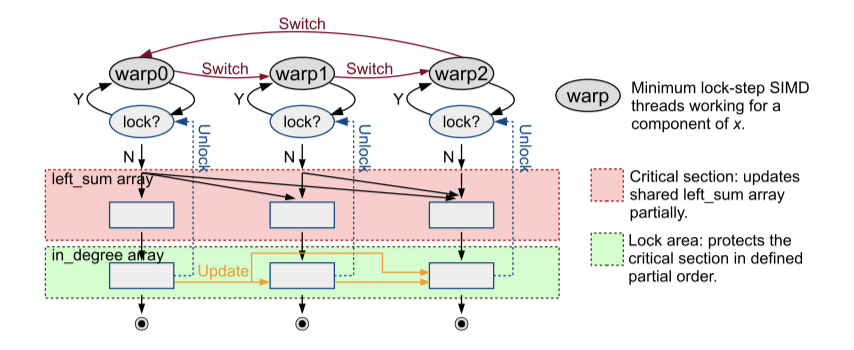
\includegraphics[width=0.7\textwidth]{sync-free.png}
    \caption{synchronization-free SpTRSV算法的示意图}
    \label{sync-free}
\end{figure}

倪鸿、刘鑫\cite{nihong2019}根据国产异构众核处理器 SW26010 体系结构的特点,针对非结构网络计算, 提出了一种基于流水线串行-局部并行思想的通用众核 SpTRSV 优化方法。首先,为了减少预处理时间,根据核心的个数,将向量 x 平均划分为多个向量块。每个向量块 x 交给一个从核进行 处理。每个从核的操作流程为:(1)等待接受来自依赖向量块的数据,直到满足进入(2)。(2)进行 x 的计算。(3)发送计算得到的 x 给需要的核心。其次,为了解决 SW26010 寄存器通讯的局限性,作者还搭建了众核通信架构。同时还有数据压缩、LDM 缓冲、访存掩盖以及数据压缩等优化。

Wang, X., Xu, P.\cite{wangFastSparseTriangular2018}等研究人员通过分析总结现有的 SpTRSV 算法,给出了一个基于生产者和消费者的统一模型,且具有一定的泛化能力。针对不同体系结构的给出了编程指导性意见。同时利用这个模型,在SW26010上提出了快速的SpTRSV算法。

\section{研究内容}

本文基于鲲鹏920处理器进行SpTRSV算法的设计与优化。研究内容包括:

\begin{enumerate} \setlength{\itemsep}{0pt}
    \item 设计一个无需预先构建任务依赖图,并且使用原子操作进行同步的SpTRSV算法。并且针对多核CPU架构的特点,以及ARMv8指令集进行优化。设计一个与华为鲲鹏平台的软硬件特性相适应的 SpTRSV 并行化方法。矩阵采用 CSC 压缩方式,将矩阵每行视作一个子任务每个任务有三种 状态:等待依赖数据,计算,结束。多个核心在任务池中并行对子任务进行如下操作:a) 自旋判断当前任务前置依赖否被满足:首先在任务入口处,自旋判断当前任务的前置依赖是否已经被满足,如果被满足则进入计算阶段。b)在计算阶段,算法对x[i],进行计算。c) 通过依赖该任务的算法,进行更新操作。
    \item 结合鲲鹏920处理器的体系结构特点以及ARMv8指令集架构进行性能优化。主要包括针对缓存的优化;针对自旋等待性能的优化,以及针对原子指令的优化。
    \item 针对NUMA架构进行优化。SpTRSV 是典型的 memory-bound 和 latency-bound 计算任务,利用 NUMA 架构可以显著提升内存带宽。目前对于 SpTRSV 算法,研究人员从任务划分、LDM 空间优化、负载均衡、自适应等角度进行了优化,取得了不错的成果。但是,缺少利用计算系统的 NUMA 特性进行优化的相关研究。我打算利用操作系统提供的libnuma编程接口,根据稀疏下三角矩阵本身是只读数据的特点,将下三角矩阵分为4个副本,分配到4个NUMA结点当中。
    \item 在SpTRSV算法中在求解x[i]时,存在的向量乘法的操作,通过使用SIMD指令提升算法的性能。编译器支持自动向量化功能,其会自动利用 NEON 属性,编译时将代码向量化。启用自动向量化功能前需要打开相应的编译选项,且并非所有代码均可向量化,其需要符合一定的编码方式和规律,以提供更多的提示信息给编译器,进一步触发编译器进行代码的向量化;也可以使用 NEON intrinsic 函数进行显示的优化。NEON intrinsic 函数是一系列 C 函数 调用,编译器可将其替换为适当的 NEON 指令或 NEON 指令序列。NEON intrinsic 函数几乎提供与编写 NEON 汇编指令相同的功能,但是将寄存器分配等工作留给编译器,以便开发人 员可以专注于算法开发。与使用 NEON 汇编指令编码相比,NEON intrinsic 方式的代码有更好的可维护性。Arm 编译器、GCC 和 LLVM 编译器都支持 NEON intrinsic
    \item 通过查阅相关文献搜集测试用的矩阵,进行正确性的验证,确保算法的正确性。结合性能分析工具,分析计算的特点,对算法进行性能的调优。最后,对并行效率和算法的可扩展性进行分析。
\end{enumerate}

\section{本文构成}

本文基与华为鲲鹏920处理以及ARMv8架构,设计高效的并行SpTRSV算法,并结合计算系统体系结构的特点进行针对性地优化。
本文的组织结构如下:

第一章绪论,主要介绍了课题背景,研究现状,研究内容,以及本文构成。在课题背景当中,我介绍了稀疏下三角矩阵求解的研究背景、应用场景及其重要意义。在研究现状当中,我分析回顾了现有国内玩研究基础、研究现状。在研究内容中,我概括性地说明研究的重点内容,及其创新特色。

第二章介绍了相关理论与技术介绍,这里我提到了稀疏线性方程组的求解常用的方法,其中稀疏下三角矩阵的求解效率的优化对直接法和不完全乔列斯基共轭梯度下降法求解线性方程组具有重要意义。接着我介绍了三种常用的稀疏矩阵压缩方式,以及我为什么选用CSC压缩方法的原因。然后我介绍了现存的SpTRSV算法,包括两种基于不同压缩格式的SpTRSV算法,以及在GPU和CPU上目前性能较好的SpTRSV算法。在第二章中,我还介绍了我所使用的优化技术及其原理,为后面算法设计打下理论基础。

第三章介绍了SpTRSV算法的设计与实现,包括如何得到下三角稀疏矩阵,如何进行正确性验证。然后我介绍了设计的SpTRSV算法和优化方法的一些具体细节,及其实现方式。

第四章我提出了算法的总体性能,一些优化方法对性能提升的效果,以及结合理论得出的分析与思考。

第五章总结与展望,对SpTRSV算法进行了总结与分析,指出了该算法的不足之处;在未来展望部分,我提出了一些仍有希望的优化思路。

\endinput
